\chapter{Megvalósítás}

\section{Grafikák elkészítése}

\subsection{Grafika megtervezése}

\subsubsection{Inspiráció}
Azok előtt, hogy nekiláttam a grafikai elemek létrehozásának, inspirációként szolgáltak az interneten elérhető rajzolási stílusok és csempekészletek. Az alapja és mintája a saját rajzaimnak a Ninja Adventure Tileset volt, amelyet Pixel-boy készített.\cite{NAT}

\subsection{Grafikus szerkesztő}

Fontos kiemelni, hogy egy "pixelart" rajz stílusról beszélünk az esetemnben, ezért fontos volt olyan rajzprogramot választanom amely minden igényemet kielégíti és könnyen kezelhető tapasztalatlan grafikusok számára is. A kiválaszott program az Aseprite volt, ebbe készítettem minden játékban megtalálható grafikát. \cite{Aseprite}

\begin{figure}[H]
    \centering
    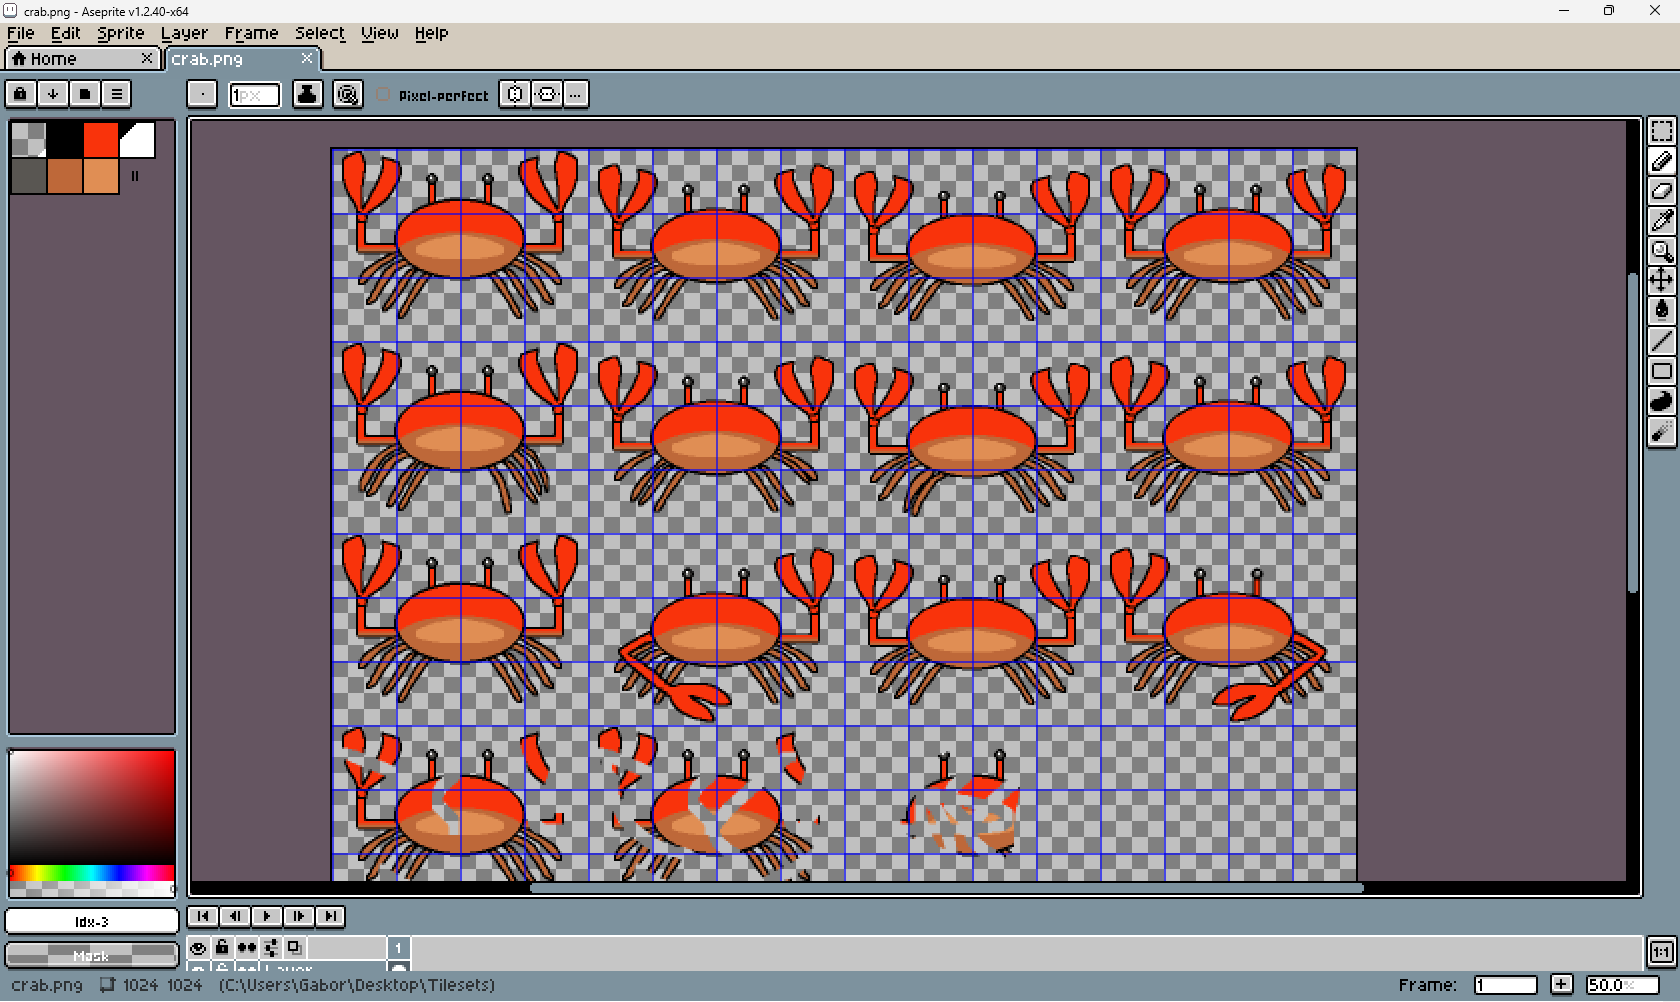
\includegraphics[width=14.0truecm]{images/Aseprite.png}
    \caption{Aseprite}
    \label{fig:Aseprite}
\end{figure}


\subsection{Rajzok elkészítése}

A rajzok elkészítése két fő részből állt, a pálya tervezéséből és a karakterek valamint a környezet kialakításából. A pálya tervezéséhez a korábban említett Ninja Adventure Tileset szolgált mintaként, melyből az összes pálya elemét saját kezűleg rajzoltam ki. A karakterek és környezet rajzainak elkészítésénél pedig meglévő rajzokat használtam inspirációként, és ezeket egészítettem ki saját kreatív ötleteimmel.

\subsubsection{Pálya}
A pályaelemek létrehozásánál kiemelkedően fontos volt figyelnem arra, hogy a csempék harmonikusan illeszkedjenek egymáshoz, ezáltal kellemes és összefüggő látványt teremtve.

\subsubsection{Entitások}
Karakterek, és szörnyek megtervezése annyiban tért el, hogy ott figyelni kellett az animációra is, hiszen élethű mozgást szerettem volna elérni. Egy ilyen mozgás animáció 4-6 képből áll, amelyeket egymás után lejátszva érhető el a kívánt hatás. Illetve mivel 4 különböző irányba tudnak haladni ezek az entitások ezért 4 különböző animációt kellett elkészítenem, amelyeket a játék során a karakter irányának megfelelően tudtam lejátszani.



\section{Pálya megtervezése}

\subsection{Tiled}
\label{subsec:Tiled}
A pálya megtervezéséhez a Tiled-et \cite{Tiled} választottam ami egy népszerű térképszerkesztő szoftver, amelyet játékfejlesztők használnak a 2D-s játékok pályáinak tervezésére és szerkesztésére. A Tiled egy nyílt forráskódú program, így ingyenesen elérhető és széles körben használt az indie játékfejlesztők körében.

Ez a szoftver lehetővé teszi a felhasználók számára, hogy könnyen létrehozzanak és testreszabjanak térképeket, amelyeket különböző játékkeretrendszerekbe integrálhatnak. A Tiled számos funkciót kínál, mint például csempekészletek használata, rétegek kezelése, objektumok és kollíziók definiálása, valamint az exportálás különböző formátumokban, például JSON vagy TMX (Tiled Map XML).

Az egyszerű és intuitív felhasználói felülete miatt a Tiled ideális eszköz a játékfejlesztők számára, akik részletes és részletekre is figyelő térképeket szeretnének készíteni játékaikhoz. Az XML alapú TMX formátum kompatibilis a legtöbb játékmotorral, így a Tiled segítségével készült térképek könnyen beilleszthetők a fejlesztési folyamatba.


\subsection{Tervezés}

Kiemelkedően fontos volt a pálya elemeit különböző rétegekre szétválasztani, ezáltal megkönnyítve a fejlesztést és az egyes részek kezelését. A háttér szolgálatában álló csempéket például két rétegre osztottam: az egyikre a talajszintet, a másikra pedig a talajon megtalálható növényzetet helyeztem el. Ezt a két réteget együttesen exportáltam PNG formátumban, amelyet a játékban háttérképként fogok használni.Fontos megjegyezni, hogy a két háttér réteget nem mentettem külön CSV fájlba. Ennek oka az, hogy ezek a rétegek olyan elemeket tartalmaznak, amelyek statikusak és nincs velük semmiféle interakció a játék során. 

Van még egy fontos réteg amik akadályként szolgálnak a játékos számára (Lásd 4.2. ábra piroskörvonal), ezeket a rétegeket a játékos nem tudja átlépni, ezáltal a játékmenetet befolyásolják.  

Lettek még rétegek létrehozva az objektumok számára, minden típúsú objektumot külön rétegen helyeztem el, így könnyen kezelhetőek és nem kell a kódban szűrést alkalmazni a különböző típusú objektumok használatakor.

\begin{figure}[H]
    \centering
    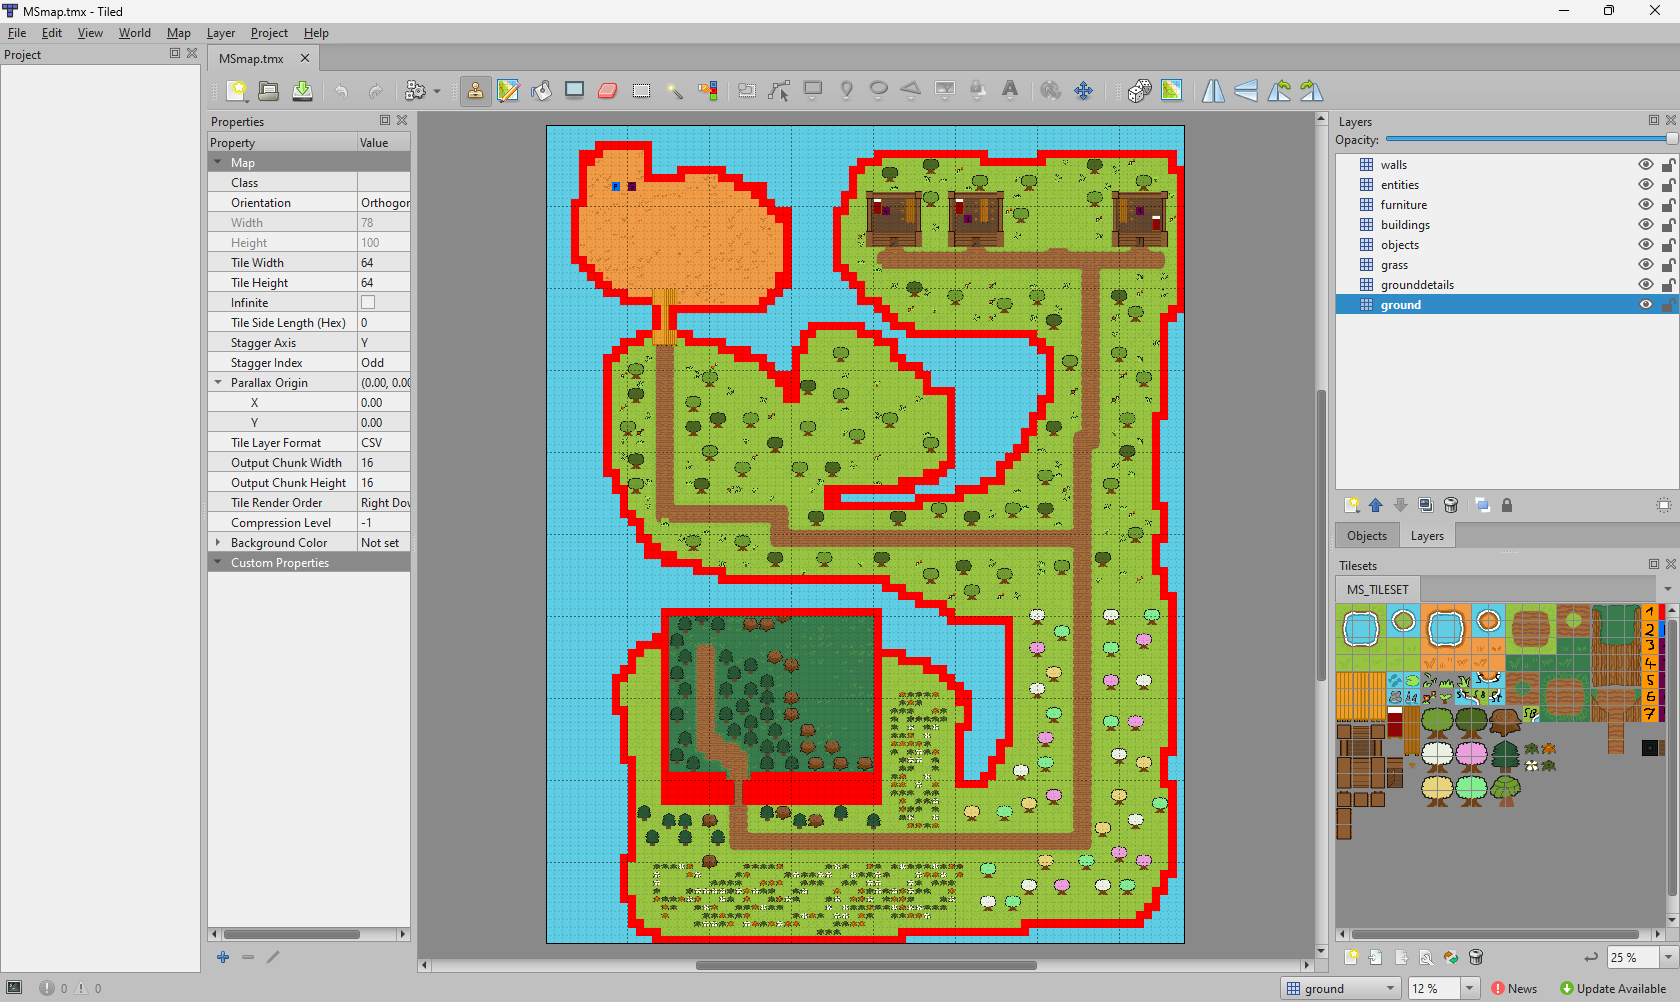
\includegraphics[width=14.0truecm]{images/Tiled.png}
    \caption{Tiled}
    \label{fig:Tiled}
\end{figure}




\section{Definiált osztályok bemutatása}
A következő szekcióban a definiált osztályok kerülnek bemutatásra.


\subsection{Settings}
Ennek az osztálynak a fő célja a beállítások kezelése egy játékban vagy alkalmazásban. Az osztály tartalmazza az alapértelmezett beállításokat, mint például a játékablak méretét, a hangerejét és egyebeket. Az osztály segítségével ezeket a beállításokat be lehet tölteni és menteni egy JSON fájlba.

Az osztályban található statikus osztályváltozók az alapértelmezett beállításokat tárolják, és a program különböző részeiben felhasználhatók. A statikus osztályváltozók előnye, hogy nem szükséges létrehozni egy példányt az osztályból, így könnyen hozzáférhetők.

Az osztály további adatokat is tartalmaz, például hangokat, grafikákat, karaktereket, ellenségeket, lövedékeket és fegyvereket. Mindezek az adatok részletezik a játékbeli objektumok tulajdonságait.

Az osztály emellett definiálja a felhasználói felület (UI) színeit és stílusait, amelyek a játék megjelenítéséhez használatosak. Ezek a színek és stílusok segítenek a felhasználói felület személyre szabásában.


\subsection{Game osztály}
Ez az osztály felelős a játék főciklusának végrehajtásáért, ami az egész játék működésének alapját képezi. Amikor a játék elindul, az alkalmazás példányosítja ezt az osztályt, és ennek a főciklusnak a futása irányítja a játékmenetet.

A 4.1. programkód részletesen bemutatja, hogyan kell megvalósítani ezt a főciklust, amely a játék lényegét adja. Ebben a kódban kezeljük a játék fő eseményeit, és gondoskodunk arról, hogy minden szükséges műveletet végrehajtsunk a játék folyamán.

Amennyiben a menürendszer visszaadja a menuenums.GAME értéket, az azt jelenti, hogy a játékot választottuk a menüből, és belépünk a játék főciklusába. Itt történik minden, a játékmenet során szükséges frissítés, eseménykezelés és kirajzolás. Itt szabjuk meg a képfrissítés mértékét is a 'self.clock.tick(Settings.FPS)' sorral, amely a másodpercenként kirajzolandó képkockák számát határozza meg.

Ez az osztály tehát létfontosságú szerepet játszik abban, hogy a játék működése zökkenőmentes és élvezetes legyen, és a kódban látható példa segítségével könnyen megérthető, hogyan történik mindez.


\begin{python}[caption={Játék főciklusa},label=py:főciklus]
    def run(self):

        while True:
            elif self.state == menuenums.GAME:
                if self.game_handler is None:
                    Sounds.play_loop('main')
                    self.game_handler = GameHandler(
                        self.user, self.save_parameters)
                for event in pygame.event.get():
                    if event.type == pygame.QUIT:
                        pygame.quit()
                        sys.exit()
                self.screen.fill(Settings.WATER_COLOR)
                self.game_handler.run()
                pygame.display.update()
                self.clock.tick(Settings.FPS)
\end{python}



\subsection{UserAuth}
Szükségem volt, hogy adatokat adatbázisba mentsek és játékmenet közben frissítsem, elérjem azokat, ezért szükséges volt implementálni egy felhasználói fiók kezelő osztályt, amely FastAPI segítségével kommunikál a MYSQL adatbázissal. 
4 fő metódussal rendelkezik, ezek a következők: felhasználónév, jelszó validálás, a bejelentkezés és regisztráció kezelése.


\subsection{MainMenu}

A játéknak elengedhetetlen része a főmenü, ami a bejelentkezés után válik elérhetővé a felhasználók számára. Biztosítok a játékosoknak offline azaz internet nélküli játszási lehetőséget, ilyenkor regisztráció és bejelentkezés nélkül használni lehet a játékot.
A főmenüben három menüpont található meg, az új játék létrehozása, meglévő mentés betöltése, illetve a beállítások. (lásd. 4.3. ábra.)   



\begin{figure}[H]
    \centering
    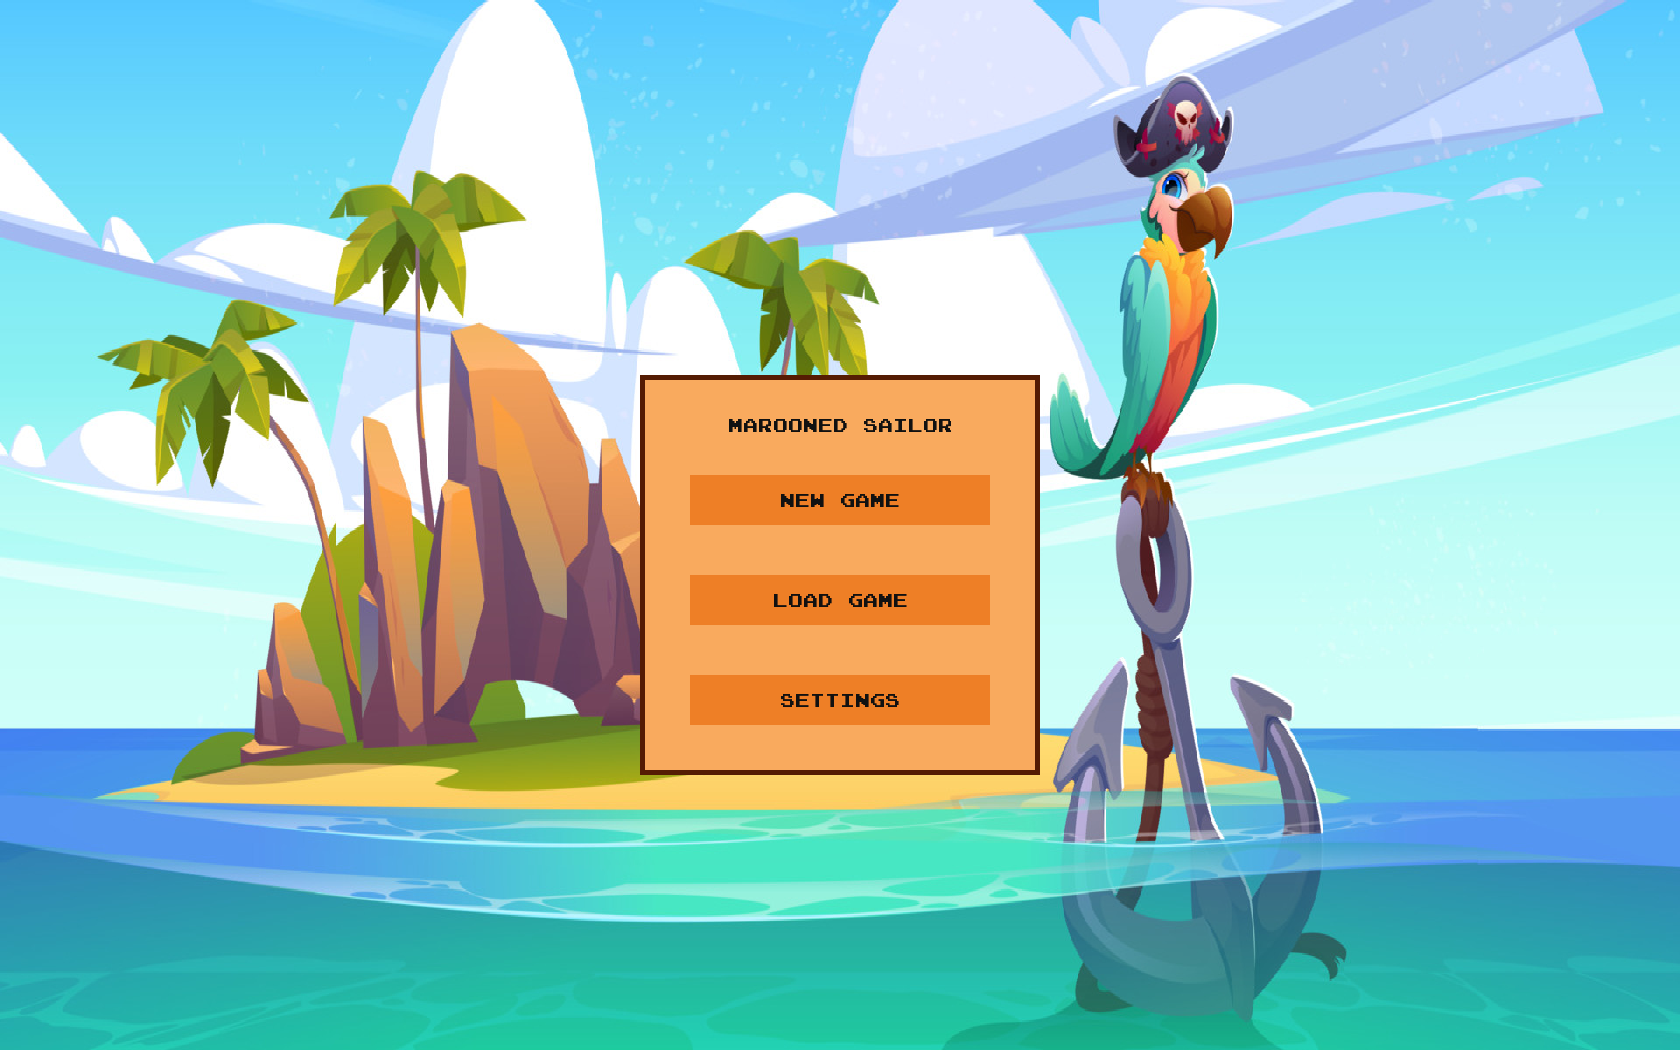
\includegraphics[width=14.0truecm]{images/mainmenu.png}
    \caption{Főmenü}
    \label{fig:Főmenü}
\end{figure}



\subsection{NewGameMenu}
Az új játék menüpont kiválasztása után a játékosnak meg kell adni a karakterének a nevét, illetve választhat különböző karakter kinézet közül. Ha be van jelentkezve a játékos, akkor van lehetősége nehézségi szintet is választani.
A nehézségi szint annyiban különbözik, hogy a "normal" módban, ha elfogy a játékos életereje, akkor a játék folytatódik tovább, újraéled egy bizonyos helyen. Viszont, ha a "challange"  módot választja akkor három funkcióval bővül a játékmenet. Az első ilyen funkció, hogy ha elfogy a játékos életereje akkor véglegesen meghal, és nem lesz lehetősége tovább folytatni azzal a bizonyos karakterrel a játékot. A második plusz funkció, hogy az összes küldetés teljesítése esetén a játék újrakezdődik amely azt eredményezi, hogy a szörnyek erősödnek, és nagyobb kihívás lesz újra végigvinni az összes küldetést. Illetve tartalmaz egy ranglista menüpontot, amely jelzi a legügyesebb játékosok hányszor tudták a "challange" mód használatával végigvinni az összes küldetést. 

\begin{figure}[H]
    \centering
    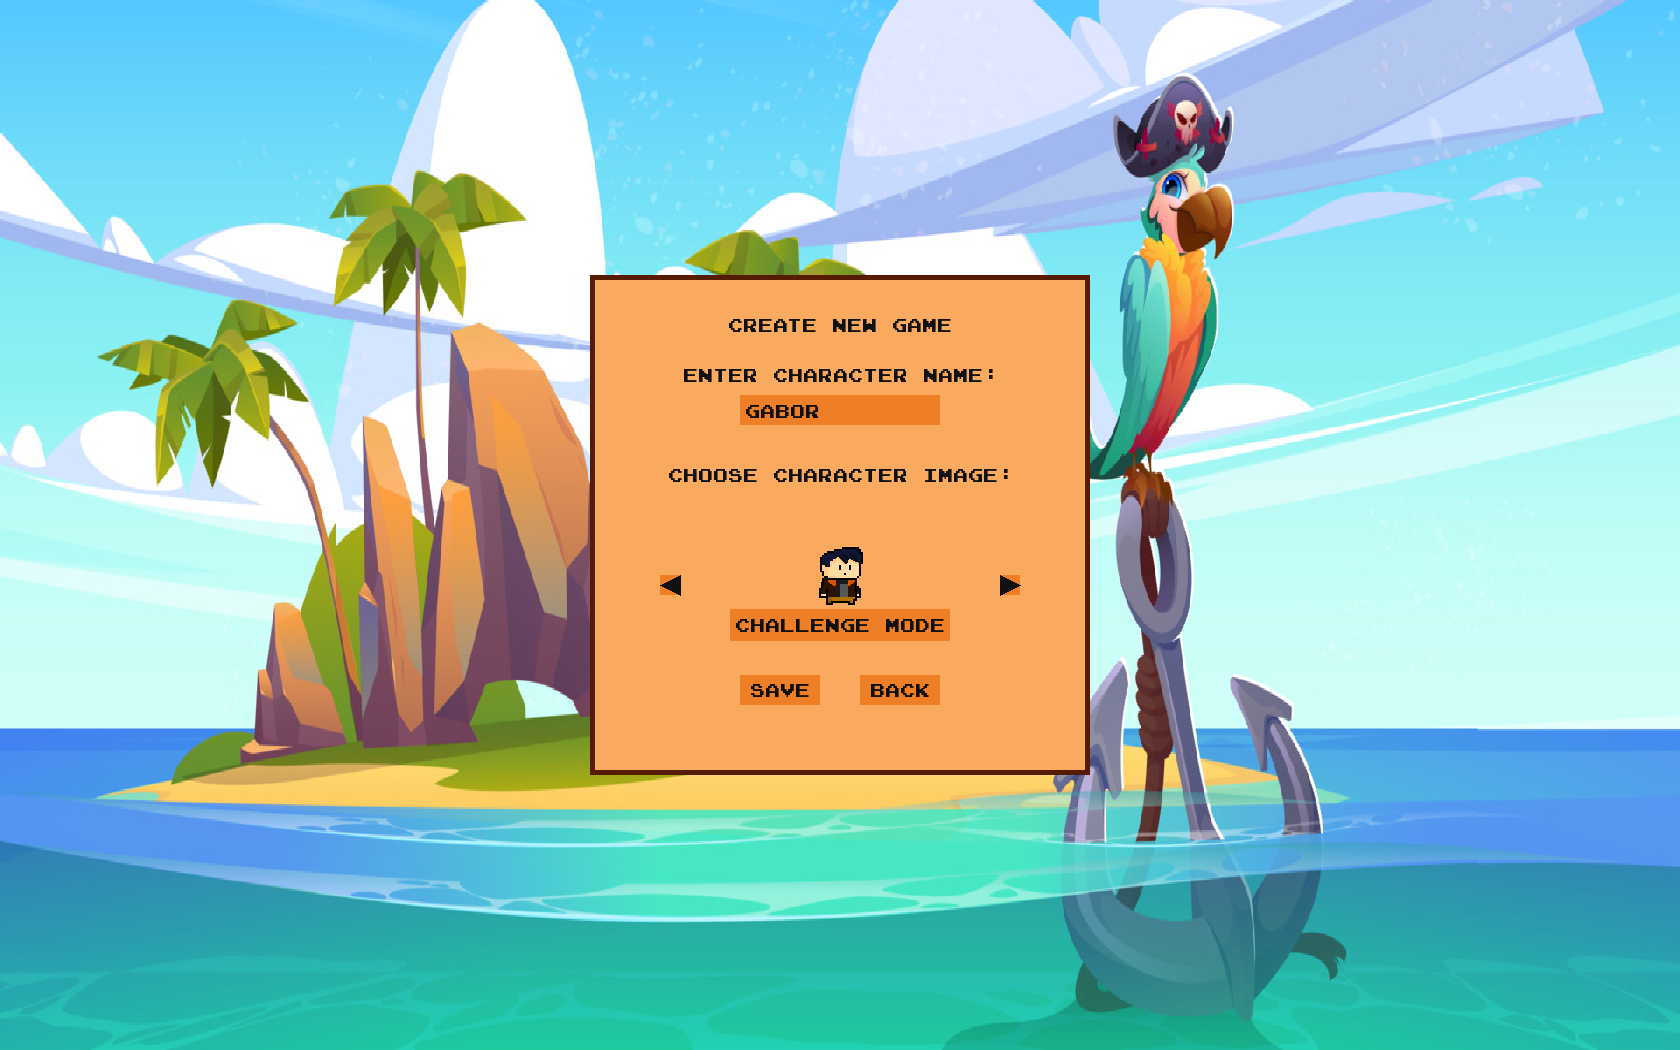
\includegraphics[width=14.0truecm]{images/newgame.png}
    \caption{Új játék létrehozása}
    \label{fig:Új játék létrehozása}
\end{figure}


\subsection{LoadMenu}
A játékosnak lehetősége van a korábban elmentett játékállás betöltésére is, amennyiben van ilyen. A betöltés után a játék folytatódik ahol abbahagyta. Egy lista elrendezésben látja a felhasználó a korábbi mentéseit. Előre rendezi az offline mentéseket a listában, és csak utánuk tölti be az online mentéseket. Egy kattintás után már be is tölti az adott játék állást.


\subsection{GameHandler}
Nagyon fontos szerepet tölt be a játék futása során, ez az osztály kezeli a mentéseket erről a következő szekcióban lesz szó bővebben. 
Továbbá a felhasználói felület kezelése és használata is itt történik. Illetve az összes játékon belüli menü funkció szintén itt példányosodik és van kezelve. Ilyen menük a játékon belüli menü, ami a pillanatálj funkcióval együtt műkdöik, a ranglista, karakter fejlesztési menü, és még az irányítások felület is ahol a felhasználó megtudja nézni, melyik gomb mire való.

\subsection{LevelHandler}
Ez a másik nagyon lényeges osztály, ez a GameHandler-ben kerül példányosításra. Feladata az világok, entitások létrehozása és kezelése. Emellett a kamera kezelés is ide tartozik. 
Ezeket a különböző felületeket Sprite Group-okba szervezve kezeli, így könnyen tudja őket elérni és frissíteni.
Legfontosabb ezek a spritegroupok közül talán a Visible Sprite Group, amely a játékos által látható felületeket tartalmazza. A kamera is ezeket rendereli ki, úgy hogy ezeket a csempéket y tengely szerint rendezi és úgy jeleníti meg, ezáltal egy hamis 3D hatást keltve.
Megtalálható még obstacle, attack, és attackable felület csoportok is amelyek a játékmenet során fontos szerepet játszanak, különböző mechanikák végrehajtásánál.


\subsection{Entity}
Ez az osztály egy szülő osztály, ami azt jelenti, hogy ebből származnak le más osztályok és felhasználják minden tulajdonságát illetve metódusait it.  
Három fontos metódussal rendelkezik az egyik a mozgás kezelése, másik egy Sin függvény alapján ad vissza 0-255 értéket, ez később a kapott sebzés kijelzésére szolgál. A harmadik metódus az ütközés érzékelésre, kezelésére szolgál.

A 4.2.-es programkód bemutatja a megvalósítását az ütközéskezelésnek. Ez lényegében úgy műkdöik, hogy nézzük az entitás mozgási irányát függőlegesen, vagy vízszintesen közlekedik, és az adott iránytól függően vizsgáljuk, hogy az entitás hitbox-a ütközik-e valamelyik akadállyal. Ha igen akkor az entitás irány szerinti hitbox-át az akadály ellenkező irányű hitbox-ához igazítjuk, így megakadályozva az áthaladást. 
\begin{python}[caption={Ütközés kezelés},label=py:Ütközés kezelés]
    def collision(self, direction):
    if direction == 'horizontal':
    for sprite in self.obstacle_sprites:
    if sprite.hitbox.colliderect(self.hitbox):
    if self.direction.x > 0:
    # moving right
    self.hitbox.right = sprite.hitbox.left
    if self.direction.x < 0:
                        # moving left
                        self.hitbox.left = sprite.hitbox.right
                        
                        if direction == 'vertical':
                        for sprite in self.obstacle_sprites:
                        if sprite.hitbox.colliderect(self.hitbox):
                    if self.direction.y > 0:
                        # moving down
                        self.hitbox.bottom = sprite.hitbox.top
                        if self.direction.y < 0:
                        # moving up
                        self.hitbox.top = sprite.hitbox.bottom
                    \end{python}

                    
                    \subsection{Player}
Ez az osztály a játékos karakterét valósítja meg, amely a játék során irányítható. A játékos karaktere egy entitás, így örökli az entitás osztály összes tulajdonságát és metódusát. Az osztály inicializálása során számos fontos adatot tárol, például a játékos nevét, karakterének azonosítóját és kezdeti pozícióját. Ezek az adatok meghatározzák a karakter kezdeti állapotát a játékban. A karakter mozgását és irányítását az osztály input metódusa kezeli. Ennek segítségével az osztály figyeli, hogy milyen billentyűk vannak lenyomva, és ennek megfelelően mozgatja a karaktert a játékban. A játékos karakter képes balra, jobbra, felfelé és lefelé mozogni a megfelelő billentyűk lenyomásával. A karakter sebessége és energiaszintje dinamikusan változik a játék során. Például a karakter gyorsabban mozoghat, ha lenyomja a "SHIFT" billentyűt, és az energia szintje csökken, miközben sprintel. Az energia idővel regenerálódik, ami lehetővé teszi a karakter számára, hogy továbbra is használja a sprintet. A játékos karakter képes támadni is, és az attack metódus meghívásával hozza létre a támadást. A támadásokat az osztály figyeli, és számítja a támadások közötti hűlési időt. A karakter fegyvere is dinamikusan változik, és a játékos lehetőséget kap a fegyver cseréjére a játék során. A karakternek van egy egészségi és energia szintje, amelyek határozzák meg túlélését a játékban. Amennyiben az egészsége nullára csökken, a karakter meghal, de van lehetőség a visszatérésre vagy újrakezdésre a játékban, attól függően, hogy a játék nehézségi szintjétől függően. A karakter számos egyéb tulajdonsággal és képességgel rendelkezik, például tapasztalati pontokkal, pénzügyi egyenleggel és teljesített küldetésekkel. Ezek a tényezők befolyásolják a játékmenetet és a karakter fejlődését. Az osztály továbbá lehetővé teszi a karakternek, hogy tárgyakat használjon és rendelkezzen egy inventáriummal. A játékos képes tárgyakat váltani és használni a játék során, ami további taktikai elemet ad a játékhoz. Összességében ez az osztály kulcsfontosságú a játékos karakter kezelésében és irányításában, lehetővé téve a játékosnak, hogy részt vegyen a játék világában és kihívásokkal nézzen szembe a karaktere fejlesztése során.
\subsection{World, Dungeon}

Egy közös szülő osztályból származnak le, ez azért fontos, hogy a különböző világokat könnyen tudjam kezelni és különböző tulajdonságokat adni nekik. Ebben az osztályban a minden világra vonatkozó lehetőségeket kezelem, ilyen például az effekteket lejátszó AnimationPlayer osztályom származtatása, hiszen azt elég egyszer definiálni és felhívni ott ahol szükséges ahelyett, hogy minden világnak lenne egy külön példánya. Továbbá ilyen opció a térképmegnyitás, és az azzal kapcsolatos összes funkció, hol található a következő küldést adó nem játékos karakter. Hiszen a játék története jelenleg teljesen lineáris, tehát egy adott sorrendben történhet csak a küldetések teljesítése. Amit még fontos megemlíteni ezzel az osztállyal kapcsolatban, az a szörnyek által dobott tárgyak, ilyen tárgy jelenleg, a tapasztalati pont, és az aranypénz. Ezeket a tárgyakat a játékos fel tudja venni, és a játék során fel tudja használni.  

\subsubsection{Pálya generáláshoz szükséges adatok}

Említettem a korábbi fejezetben, a pálya megtervezését a \textbf{Tiled}-el végeztem. (Lásd \ref{subsec:Tiled}) 
Első megközelítésemkor CSV (vesszővel elválaszott értékek) fájl formátumba mentettem ki a tervezőben létrehozott rétegeket. Egy ilyen dokumentum úgy néz ki, hogy ahova nem helyeztem le a tervezőben objektumot ott '-1' érték szerepel, ellentétben ahol van érték ott a Tiled-ben betöltött és feldarabolt csempekészlet azonosító számai kerültek a dokumentumba. Ezt úgy kell elképzelni mint egy nagy mátrixot. Az utolsó pillanatokig ezt a megközelítést alkalmaztam, hiszen ha már kész volt és működött miért változtattam volna rajta. Végül mégis visszatértem erre a kérdéskörre és készítettem az alább olvasható kis egyszerű átalakító szkriptet. (Lásd \ref{py:csvtodict}) Ennek funkciója, a sok felesleges '-1' értéket kiszűrni, hogy a program futása közben, ne kelljen a betöltésnél rengeteg felesleges összehasonlítást végezni. Ezt úgy oldottam meg, hogy készítettem python szótárat a csempe azonosító számából illetve annak a csv mátrixban elhelyezkedő koordinátáiról. (Lásd \ref{py:átalakított struktúra})


\begin{python}[caption={csvtodict},label=py:csvtodict]
    import csv
    import json
    
    csv_file = "new_map\MSmap._dungeonentrance.csv"
    map_data = []
    
    with open(csv_file, newline='') as csvfile:
        csv_reader = csv.reader(csvfile)
    
        for i, row in enumerate(csv_reader):
            for j, value in enumerate(row):
    
                value = int(value)
    
                    map_data.append({"i": i, "j": j, "value": value})
    
    python_file = "world_dungeonentrance"
    
    with open(python_file, 'w') as pyfile:
        pyfile.write("map_data = ")
        json.dump(map_data, pyfile, indent=4)
    
    print(f"Dictionary saved to {python_file}")
    
\end{python}


\begin{python}[caption={Minta az átalakított struktúrára}, label=py:átalakított struktúra]
    {
        "i": 3,
        "j": 41,
        "value": 125
    },
\end{python}


\subsubsection{Pálya generálás}

Most, hogy már grafika és a pálya rétegek elkészültek amik ki lettek exportálva, ideje ezeket az adatokat egyesíteni és megjeleníteni a játékban. Ezt több lépésben valósítottam meg, először is a képeket be kell tudnom olvasni, ezt az os könyvtár walk függvényének segítségével oldottam meg. Miután sikerült bejárni a mappát, előállítom az egyes képekhez vezető útvonalat, és ezután a pygame.image.load függvényével betöltöm a képeket. Ezt követően a képeket egy listába helyezem, amelyet később fel tudok használni a kirajzoláshoz. Másik ilyen fontos lépés a pálya rétegek beolvasása, amelyet a korábban említett szótárak segítségével valósítottam meg. Ezután egy ciklusban végig iterálva a szótáron, a képek listájából kiválasztom a megfelelő képet, és a megfelelő koordinátákat amiket segítségével példányosítom a Tile (csempe) osztályt később ennek segítségével végzem el a kirajzolást. Mivel a szótárak között szerepel az entitásokra vonatkozó réteg is, ezért azokat is az előbb említett iterációban kezelem, és példányosítom a hozzájuk tartozó osztályokat azonosító alapján szűrve.

Készítettem egy kis függvényt, a pálya létrehozásának idejének meghatározására. Ez azért volt fontos, hogy megtudjam határozni, hogy a szótár használata jobb megoldás-e, mint a CSV fájl. A két megoldás esetében a következő eredményeket kaptam:

Szótár esetében:
\begin{verbatim}
    Futási idő: 108.64 ms
\end{verbatim}
CSV fájl esetében:
\begin{verbatim}
    Futási idő: 879.92 ms
\end{verbatim}

Tehát elmondható, hogy ez a változtatás jelentősen felgyorsította a pálya létrehozását, ezáltal a játék betöltési ideje is csökkent.

\subsection{Enemy}


\chapter{tutorial}



Ez a fejezet mutatja be a megvalósítás lépéseit.
Itt lehet az esetlegesen előforduló technikai nehézségeket említeni.
Be lehet már mutatni a program elkészült részeit.

Meg lehet mutatni az elkészített programkód érdekesebb részeit.
(Az érdekesebb részek bemutatására kellene szorítkozni.
Többségében a szöveges leírásnak kellene benne lennie.
Abból lehet kiindulni, hogy a forráskód a dolgozathoz elérhető, azt nem kell magába a dolgozatba bemásolni, elegendő csak behivatkozni.)

A dolgozatban szereplő forráskódrészletekhez külön vannak programnyelvenként stílusok.
Python esetében például \mref{py:test}ban látható egy formázott kódrészlet.
\begin{python}[caption={Python példa},label=py:test]
    import sys
    
    if __name__ == '__main__':
    pass
\end{python}

A stílusfájlok a \texttt{styles} jegyzékben találhatók.
A stílusok között szerepel még C++, Java és Rust stílusfájl.
Ezek használatához a \texttt{dolgozat.tex} fájl elején \texttt{usepackage} paranccsal hozzá kell adni a stílust, majd a stílusfájl nevével megegyező környezetet lehet használni.
További példaként C++ forráskód esetében ez így szerepel.
\begin{cpp}
    #include <iostream>
    
class Sample : public Object
{
    // An empty class definition
    }
\end{cpp}
Stílusfájlokból elegendő csak annyit meghagyni, amennyire a dolgozatban szükség van.
Más, C szintaktikájú nyelvekhez (mint például a JavaScript és C\#) a Java vagy C++ stílusfájlok átszerkesztésére van szükség.
(Elegendő lehet csak a fájlnevet átírni, és a fájlban a környezet nevét.)

Nyers adatok, parancssori kimenetek megjelenítéséhez a \texttt{verbatim} környezetet lehet használni.
\begin{verbatim}
    $ some commands with arguments
    1 2 3 4 5
    $ _
\end{verbatim}

A kutatás jellegű témáknál ez a fejezet gyakorlatilag kimaradhat.
Helyette inkább a fő vizsgálati módszerek, kutatási irányok kaphatnak külön-külön fejezeteket.
